\documentclass{article}

\usepackage{graphicx}
\begin{document}


\title{Fugu}
\author{Brad Aimone, William Severa, Craig Vineyard}

\maketitle


\section{Introduction}

This document summarizes the notes from the Fugu Week by BA, WS, and CV at the end of September

\section{Overview of Fugu}

\subsection{Goal of Fugu}
The primary goal of Fugu is to provide a general scientific computing user access to emerging neuromorphic hardware --- specifically \textit{spiking} neuromorphic hardware --- by providing an accessible library of functions that Fugu provican map into neural hardware

Fugu provides the following core capabilities 
\begin{itemize}
\item \textbf{API to conventional programming environments (i.e., C++, Python)} 
\item \textbf{A functional \textit{intermediate representation} of spiking neural algorithms}
\item \textbf{Outputs to neural hardware compilers or Fugu's reference simulator}
\end{itemize}

\subsection{API}

The goal of the API for Fugu will be to make the construction of a Fugu algorithm be readily called from C++ or Python.  In theory, all of the spiking algorithm requirements and processing should be transparent to a user; such that they only have to call a function with standard I/O protocols; not unlike CUDA.


\subsection{Intermediate Representation}

The primary contribution of Fugu is the managed IR between higher-level coding environments and low-level neuromorphic hardware and their compilers.  This IR consists of three components that, during compilation, provide the connection between the API and the compiler output: a library of \textit{SNA Modules}, a collection of algorithms for linking SNA Modules, and the combined application graph output.  

The IR of Fugu exists within Python, and it leverages the NetworkX libary to construct and manage the neural circuits that will be generated and combined during Fugu operation.

\subsubsection{Library of SNA Modules}
Each spiking neural algorithm (SNA) within Fugu is termed a Module (for the time being).  Importantly, the algorithms that are contained within Fugu are not explicit neural circuits, but rather the algorithms that can generate the appropriate neural circuit for a given application.  

For example, we consider the constant-time 1-dimension max cross-correlation algorithm by Severa et al., ICRC 2016.  That algorithm compares two binary vectors of length $n$ by having a dedicated neuron within an intermediate layer calculate each potential off-set, requiring an intermediate layer of size $n^2$.  Subsequently, an output layer, sized $2n-1$ samples that intermediate layer to determine the relative shift between inputs that yields the maximal overlap.  

As the description shows, the exact neural circuit needed is highly specific to $n$.  In addition, the resulting circuits have other important properties that will be necessary at later Fugu stepts.  For instance, for the constant-time algorithm, the inputs are provided all at the same time ($T_{in} = 1$), and the output is always a single time-step ($T_{out} = 1$) arriving two time steps later ($D = 2$).  An alternative version of this algorithm streams the inputs in over time and uses delays to make the same computation with fewer neurons, albeit at an extended time cost, a characteristic that will produce different neural circuit and associated metadata.  It is also important to note that this metadata may be a function of input parameters as well --- for instance in the matrix-multiplication application described in Parekh et al., SPAA 2018, there is a version of the algorithm whose depth is $O(log log n)$, where $n$ is the size of the largest matrix dimension.  

A schematic of the module is shown in figure \ref{module}. The properties of each module within Fugu are:

\begin{itemize}
\item $N_{in}$ -- number of input neurons
\item $T_{in}$ -- time length of inputs (how long do inputs stream in).  =inf if streaming
\item $N_{out}$ -- number of output neurons
\item $T_{out}$ -- time length of output.  = inf if streaming
\item $D$ -- circuit depth, corresponding to how many global timesteps must pass for the input at t=1 to reach  
\end{itemize}

To exist within Fugu, each of the modules must be able to take instructions from the Fugu environment and produce the appropriate neural circuit NetworkX graph per the necessary scales and timings.  These circuits are referred to as \textit{local circuits}, and are standalone circuit SNAs for computing the requisite function.  

Further, at build time, only one of the modules may have a well-defined set of parameters.  The parameters of other modules are dependent on that module's inputs. So each module must also have a function \textbf{returnParameters($N_{in}$)}, which returns, for that module, the appropriate size of that module when the input size is defined.  This function will be of importance in linking the modules.

\begin{figure}
	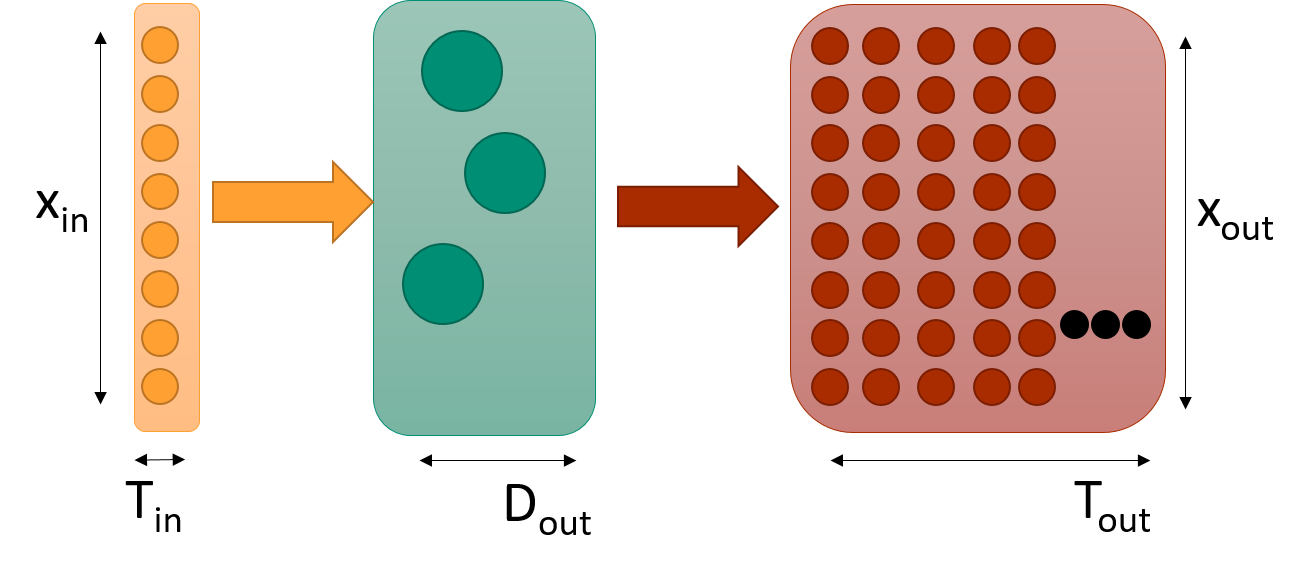
\includegraphics[width=5in]{module_simple.png}
	\label{module}
	\caption{Fugu Module}
\end{figure}

The set of required functions for each module are as follows:

\begin{itemize}
	\item \textbf{returnParameters($N_{in}$)} returns $N_{out}, T_{in}, T_{out}, D$
	\item \textbf{buildModule($N_{in}, N_{out}, T_{in}, T_{out}, D$)} returns NetworkX graph of algorithm at desired size
\end{itemize}

\subsubsection{Linking code to combine local circuits into global circuit}

Once the individual Modules are identified to generate all of the required local circuits, a secondary routine is required to appropriately scale the modules, generate the circuits, and link these output NetworkX graphs together into a larger unified global circuit.  There are two primary challenges and a number of routine steps that require care for linking these circuits together.  

\begin{itemize}
\item \textbf{Align sizes of modules}.  Each model has an input size $N_{in}$ and an output size $N_{out}$, and in order for two modules to be compatible with one another \textit{serially}, then it is necessary that the downstream module is scaled appropriately to generate a graph suitably sized to take the outputs.  
\item \textbf{Align timings of modules}.  Each of the modules has associated with it a $T_{in}$, $T_{out}$, and a $D$.  If modules are intended to run in \textit{parallel}, the difference in timings and depths may require that an additional \textit{delay circuit} is instantiated on one of the pathways to ensure that the circuit is appropriately timed.
\end{itemize}

\textbf{Stage 1: Normalizing graph sizes}

As the first point above states, any serial alignment of multiple Fugu modules will at minimum require that the I/O of the modules are compatible with one another.   As only the first modules have defined sizes (by whatever input data is identified at the onset), Fugu must deduce the sizes of all subsequent modules.  A general scheme is shown in Figure \ref{serial_link}. 

\begin{figure}
	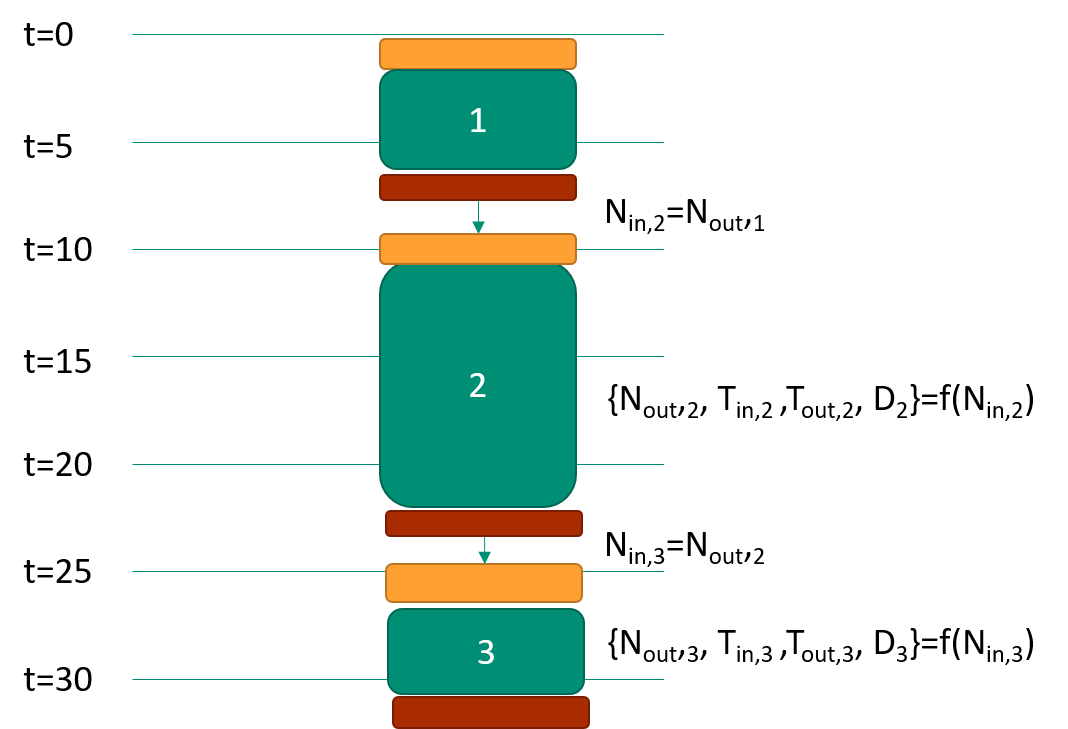
\includegraphics[height=3in]{module_link_serial.png}
	\label{serial_link}
	\caption{Normalizing module sizes}
\end{figure}

This sizing algorithm is relatively straight forward.  We assume that the first Fugu module has a defined set of size parameters $[N_{in}, N_{out}, T_{in}, T_{out}, D]_1$, and that any module can be fully defined by setting its input size.  (\textbf{Note: we may also want to flag different depth versions of some algorithms}).  After the graph for the first module is built, we move to the second module.  Here, we take $N_{in,2}$ to be equal to $N_{out,1}$, and then we retrieve the other size parameters for module two by calling \textbf{returnParamaters} with $N_{in,2}$ for module 2, and then building that module.  So long as the module sequence is serial, we can proceed in this manner.  

If there is any branching the module sequence, the sizing clearly will depend on the upstream module in terms of I/O; regardless of what the indexing may be.  Within each branch, the serial sizing can proceed as above.  

\textbf{State 2: Normalizing the architecture timing}

So long as the structure of the anticipated combined Fugu network is serial, timings do not have to be worried about.  However, once there is a branch in the code, whereby two circuits will then run in parallel for a period of time, only to be brought back together, it becomes necessary to include some additional steps to keep the overall computation in synchrony (Figure \ref{parallel_link}).

As the branches may be indexed arbitrarily and the time or depth of a module may be undetermined until its overall size is identified, it is unknown at the start of Fugu which branch will be the limiting factor in terms of time.  So once Stage 1 above is completed and the sizes of each module is defined and the component graphs are produced, we must then determine the longest branch. (for i... Nbranches; find longest).  This longest branch is the reference length that all other branches must match.  Once this \textit{branch depth} is found, we then work through each of the other branches to make the depths equivalent.

Two options are possible at this point.  First, we can simply add a delay block - most simply a set of repeater neurons that spike with a delay of whatever the difference is.  Most simply, this delay block could be at the end of the branch. However, there is likely a benefit to load balance over time; the delays will be relatively cheap in terms of computation, and thus they can perhaps be staggered at different times of each branch to keep the overall network activity at a roughly comparable level.  

The second approach is more subtle.  Many of the SNAs being developed can be tailored to use fewer neurons if more time is available.  This time-space tradeoff is generally biased towards the faster algorithm; however in cases where a module with such a tradeoff sits within a branch with "free-time" so to speak, it is possible, and perhaps even advantageous, to represent that module in a more time-costly, space-efficient manner that reduces the overall neuron footprint of the model.

For this second approach, it may be useful to have access to an "alternate" graph, or at least access to some form of metadata that will inform Fugu whether that is an option.

\textbf{Stage 3 - Link graphs together}

Once the architecture has been fine-tuned to keep delays constant and the graphs are all produced with the required sizes, it is then necessary to combine the graphs into one large graph.  This would likely best proceed serially through the set of modules. The key, as shown in Figure \ref{combined}, is to replace the input nodes of the downstream graph with the output nodes of the upstream graph.  

One note here is that the dynamics may likely need to be normalized, at least for these overlapping populations.




\begin{figure}
	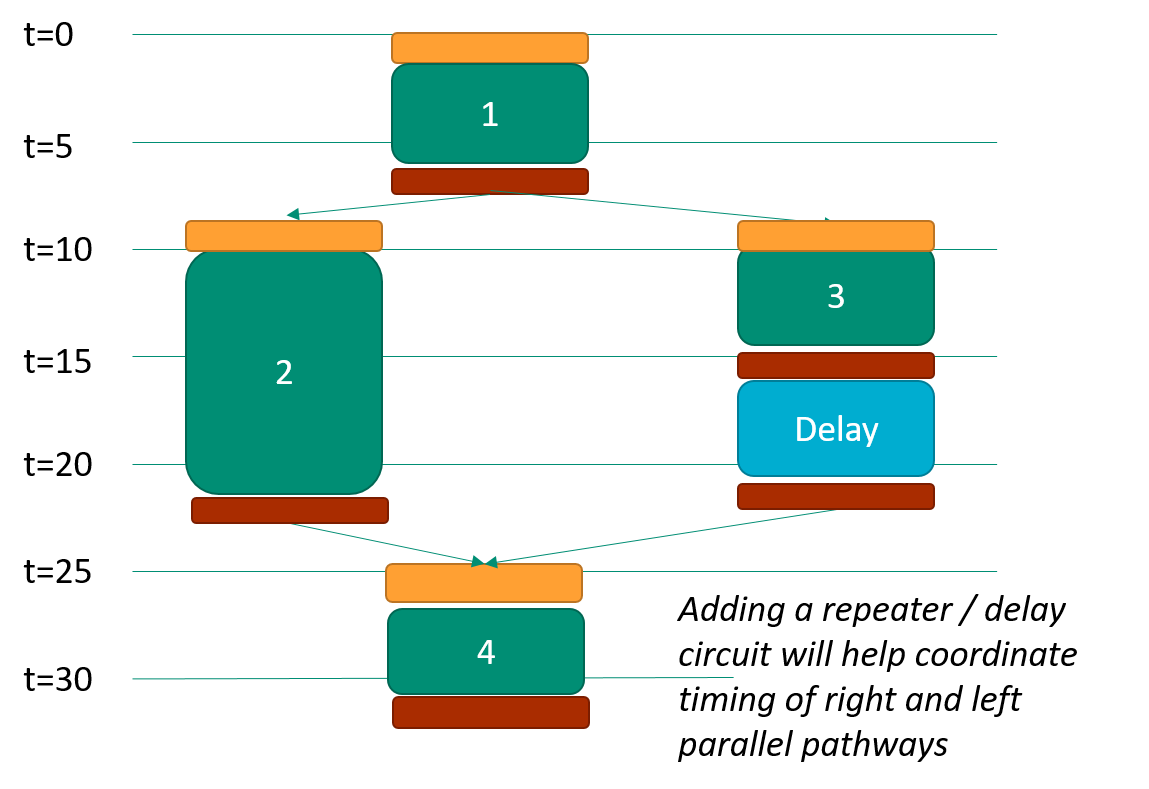
\includegraphics[height=3in]{module_link_parallel.png}
	\label{parallel_link}
	\caption{Adding a delay to synchronize Fugu branches}
\end{figure}

\begin{figure}
	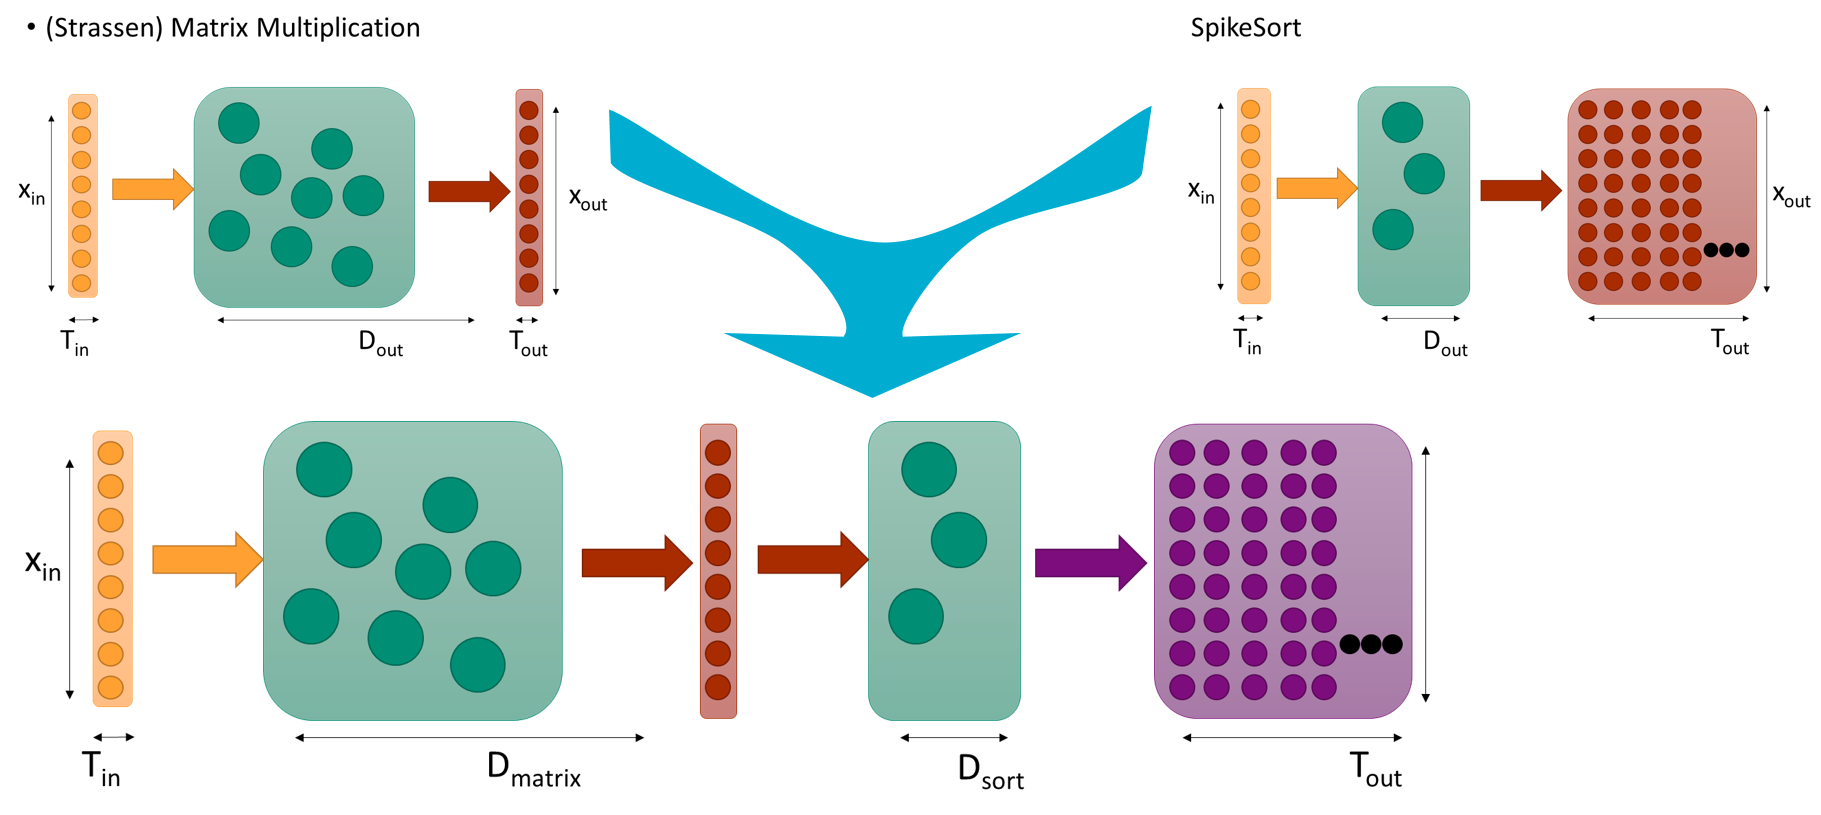
\includegraphics[width=5in]{module_combined.png}
	\label{combined}
	\caption{Combined Modules}
\end{figure}



\subsubsection{Output}
The output of Fugu will be a single NetworkX graph that fully describes the spiking neural algorithm.  The \textbf{edges} of this graph will be the synapses of the model, and will accordingly have weights associated with them as attributes.  The \textbf{nodes} of this graph will be the neurons of the model, and will accordingly have dynamics parameters associated with them.  Additionally, some parameters, such as learning rates, additional dynamical states, etc. may be included within the attributes.

\begin{itemize}
	\item Edges = synapses
	\begin{itemize}
		\item source, target (required)
		\item weight (required)
		\item plasticity attributes (optional)
	\end{itemize}
	\item Nodes = neurons
	\begin{itemize}
		\item id (required)
		\item dynamics parameters (required)
	\end{itemize}
		
\end{itemize}


\subsection{Compiler}

There output of the Fugu linking process is a single NetworkX graph with described dynamics within the nodes.  In principle, this description, along with metadata describing the I/O and a few other parameters, should be sufficient to fully describe the spiking neural algorithm.  Of course, different neuromorphic hardware platforms will have differing requirements on how networks should be represented as well as distinct constraints, such as graph restrictions or specialized neural dynamics.  

Fugu will come with three general options.  First, Fugu will come with a \textbf{reference simulator}which will be guaranteed to run any Fugu-compatible algorithm.  The reference simulator will not be optimized for speed or performance, but it will provide a rough-order-of-magnitude ability to benchmark performance of Fugu graphs.  The second type of output will be \textbf{ONNX network descriptions}, whereby ONNX-compatible Fugu graphs (likely a narrow restricted set that look like feed-forward ANNs) can be output as ONNX files and thus readily transferred to ONNX-compatible hardware.  The final output, and the one most intended for Fugu operationally, is a suite of \textbf{neuromorphic hardware-specific compilers}.  Likely, this step will require a different compiler tool for each hardware platform; although for some (such as SpiNNaker and sPyNNaker), existing tools may be able to be used with relatively modest translation.

\subsubsection{Reference Simulator}

The reference simulator will be a very straightforward python simulation of the NetworkX graph with leaky-integrate and fire dynamics.  It is intended to fully capture the full representational capacity of what Fugu networks can represent; so if Fugu is extended in any meaningful way (e.g., adding learning rules), the reference simulator must account for that.

The goal of the reference simulator is to enable the following:

\begin{itemize}
\item Validation of Fugu NetworkX outputs
\item Provide ballpark estimates for performance
\item Enable and apples-to-apples comparison between spiking algorithms

\end{itemize}

\subsubsection{ONNX}

...description of why we need ONNX compatibility here...


\section{Algorithms within Fugu}
\subsection{Algorithms we have...}
\begin{itemize}
	\item Numerical Kernels
	\begin{itemize}
		\item Matrix-Matrix Multiplication  (\textit{Parekh et al., SPAA})
		\item Vector-Matrix Multiplication
		\item Cross-correlation (\textit{Severa et al., ICRC})
		\item Triangle counting (\textit{Parekh et al., SPAA})
	\end{itemize}
	\item Data Measures
	\begin{itemize}
		\item L1-norm (\textit{Severa et al., ICRC})
		\item Counters (\textit{Severa})
		\item SpikeMax, SpikeMin, SpikeSort (\textit{Verzi et al., Neural Computation})
		\item K-nearest neighbor (\textit{Vineyard})
		\item Djikstra (\textit{Parekh, Severa})
	\end{itemize}
	\item Data Manipulation
	\begin{itemize}
		\item Low-pass Filter (\textit{Severa})
		\item Convolutions (\textit{Severa})
	\end{itemize}
	\item Application algorithms
	\begin{itemize}
		\item Whetstone (\textit{Severa et al., submitted})
		\item Monte Carlo Random Walk (\textit{Severa et al., IJCNN})
	\end{itemize}

\end{itemize}
\subsection{Algorithms we need...}
\begin{itemize}
	\item Numerical Kernels
	\begin{itemize}
		\item Basic Arithmetic (add, substract, multiply, divide, etc)
	\end{itemize}
	\item Data Measures
	\begin{itemize}
		\item
	\end{itemize}
	\item Data Manipulation
	\begin{itemize}
		\item Delay / Repeat
		\item Code remapping (spatial --> temporal, etc.)
		\item Hashing
	\end{itemize}
	\item Application algorithms
	\begin{itemize}
		\item Random Forest
	\end{itemize}

\end{itemize}

\subsection{Algorithms we could have...}
\begin{itemize}
	\item Numerical Kernels
	\begin{itemize}
		\item Fourier
		\item Binary dot product
		\item Matrix inversion
	\end{itemize}
	\item Data Measures
	\begin{itemize}
		\item
	\end{itemize}
	\item Data Manipulation
	\begin{itemize}
		\item High-pass filter
	\end{itemize}
	\item Application algorithms
	\begin{itemize}
		\item Graph 500 suite
		\item Support Vector Machines
		\item SpikeART
		\item 
	\end{itemize}

\end{itemize}




\end{document}